\bfsection{平成31年度 専門科目}

\bfsubsection{問1}
\barquo{
$\R[X,Y]$を変数$X,Y$に関する実数係数の$2$変数多項式環とする。$I$を$X^2 + Y^2$で生成された$\R[X,Y]$のイデアルとする。$A = \R[X,Y]/I $とおく。このとき、以下の問に答えよ。
\begin{description}
  \item[(i)] $A$は整域であることを示せ。
  \item[(ii)] $A$の商体を$K$とおき、$A$の$K$における整閉包を$B$とおく。$A$加群としての$B$の生成系を一組与えよ。
\end{description}
}
\begin{sol} ${}$
  \begin{description}
    \item[(i)] $\R[X,Y]$はUFDなので、$X^2 + Y^2$が既約元であることを示せばよい。可約であると仮定する。そうするとある実数$a,b,c,d $が存在して$X^2 + Y^2 = (aX + bY)(cX + dY)$が成り立つことになるが、そうすると$ac - 1 = ad + bc = bd - 1 = 0$でなくてはならない。これは$a,b,c,d$が実数であったことに矛盾。よって$X^2 + Y^2$は既約元であり、$I \subset \R[X,Y]$は素イデアル。
    \item[(ii)] $a = Y/X$とする。$a^2 + 1 = 0$なので$a \in B$である。$B = A[a]$を示そう。それには、$A[a]$が整閉であることを示せば十分である。$\R$代数の準同形$\vp \colon \R[X,\I] \to A[a]$を$\vp(\I)=a, \vp(X)=X$で定める。これはwell-definedであり、あきらかに全射。$f \in \Ker \vp$とする。
    \[
    f = \sum_{i=0}^n (a_i+\I b_i) X^i
    \]
    と表せる。そうすると
    \[
    0 = \sum_{i=0}^n a_i X^i + Y \sum_{i=1}^n b_i X^{i-1}  + b_0 \f{Y}{X}
    \]
    である。ここから$f=0$が導かれる。よって$\vp$は同型であり、$A[a] \cong \R[X,\I] \cong \C[X]$である。とくに$A[a]$は整閉だから$B = A[a]$が示された。
  \end{description}
\end{sol}




\bfsubsection{問5}
\barquo{
$\C$の部分空間
\[
X = \setmid{1- e^{i\grt} \in \C }{0 \leq \grt < 2\pi} \cup \setmid{-1 + e^{i\grt} \in \C}{0 \leq \grt < 2\pi }
\]
を考える。整数$p,q$に対して、写像$f \colon X \to X$を
\begin{align*}
  f(1- e^{i\grt}) &= -1 + e^{ip\grt} \\
    f(-1 + e^{i\grt}) &= 1 - e^{iq\grt}
\end{align*}
で定め、$X \tm [0,1]$に
\[
(x,0) \sim (f(x),1)
\]
($x \in X$)で生成される同値関係$\sim$を与える。商空間$Y = (X \tm [0,1])/ \sim$の整数係数ホモロジー群を計算せよ。
}
\begin{sol}

セル複体を使ってホモロジーを求めよう。空間$Y$を直接書くことは難しいが、次のようなものを想像することはできる。

\begin{center}
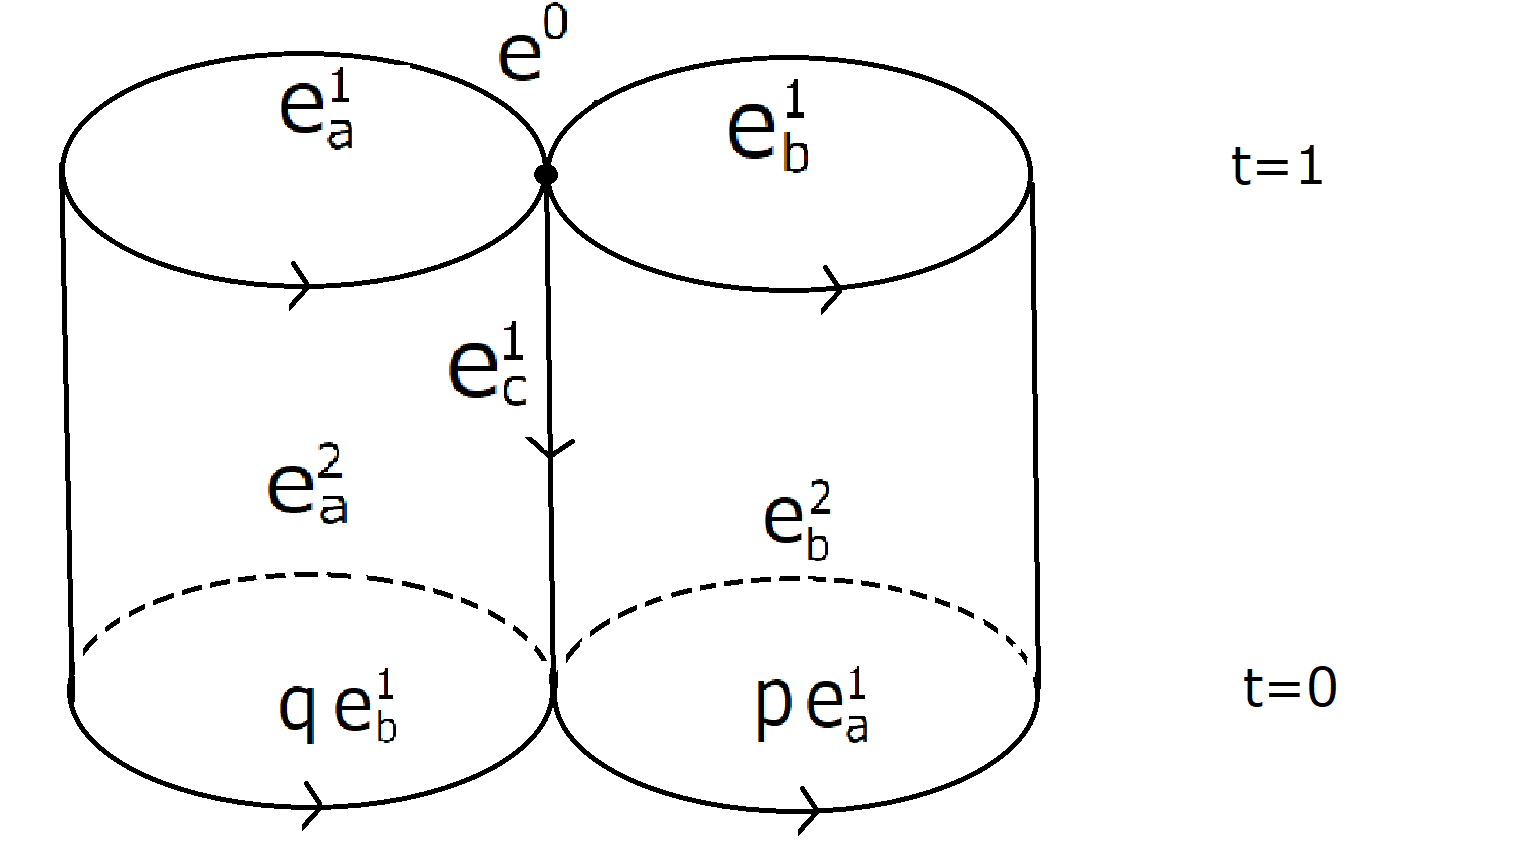
\includegraphics[width=5cm]{H31expert05_01.png}
\end{center}

この対になった円筒は、$X \tm I$および$Y$を表している。上下の円盤に見える部分は円周であり、ちくわを2つくっつけたような形をしている。側面も輪郭しか書かれていないが、面になっている。垂直方向が$I$成分を表しており、上が$t=1$で下が$t=0$であるものとしよう。また右を実軸のプラス方向、奥を虚軸のプラス方向とする。上部にある点は原点を表す。図に$e$と書かれているのはセルである。それぞれ具体的には次のように与えられる。
\begin{align*}
  e^0 &= (0,1) \\
  e^1_a &= \setmid{ (-1+e^{i\grt},1) }{0 < \grt < 2\pi } \\
  e^1_b &= \setmid{ (1-e^{i\grt},1) }{0 < \grt < 2\pi } \\
  e^1_c &= \setmid{ (0,t) }{0 < t < 1 } \\
  e^2_a &= \setmid{ (-1+e^{i\grt},t) }{0 < \grt < 2\pi , 0 < t < 1 } \\
  e^2_b &= \setmid{ (1-e^{i\grt},t) }{0 < \grt < 2\pi , 0 < t < 1 }
\end{align*}
このとき、次に注意する。
\begin{align*}
  e^0 &= (0,0) \\
  pe_a^1 &= \setmid{ (1-e^{i\grt},0) }{0 < \grt < 2\pi } \\
  qe_b^1 &= \setmid{ (-1+e^{i\grt},1) }{0 < \grt < 2\pi }
\end{align*}
さて以上の準備の下セル複体のホモロジーを計算しよう。$Y$の$0$セル、$1$セル、$2$セルの数はそれぞれ$1,3,2$個なので
\[
\xymatrix{
0 \ar[r] & \Z^2 \ar[r]^{\del} & \Z^3 \ar[r]^{\grs} & \Z \ar[r] & 0
}
\]
という図式に表されるような状況になっている。まず$\grs$だが、$0$セルはただひとつしかないのでこれはゼロ写像である。よって$H_0(Y)=\Z$がわかる。
次に$\del$を計算する。次の図

\begin{center}
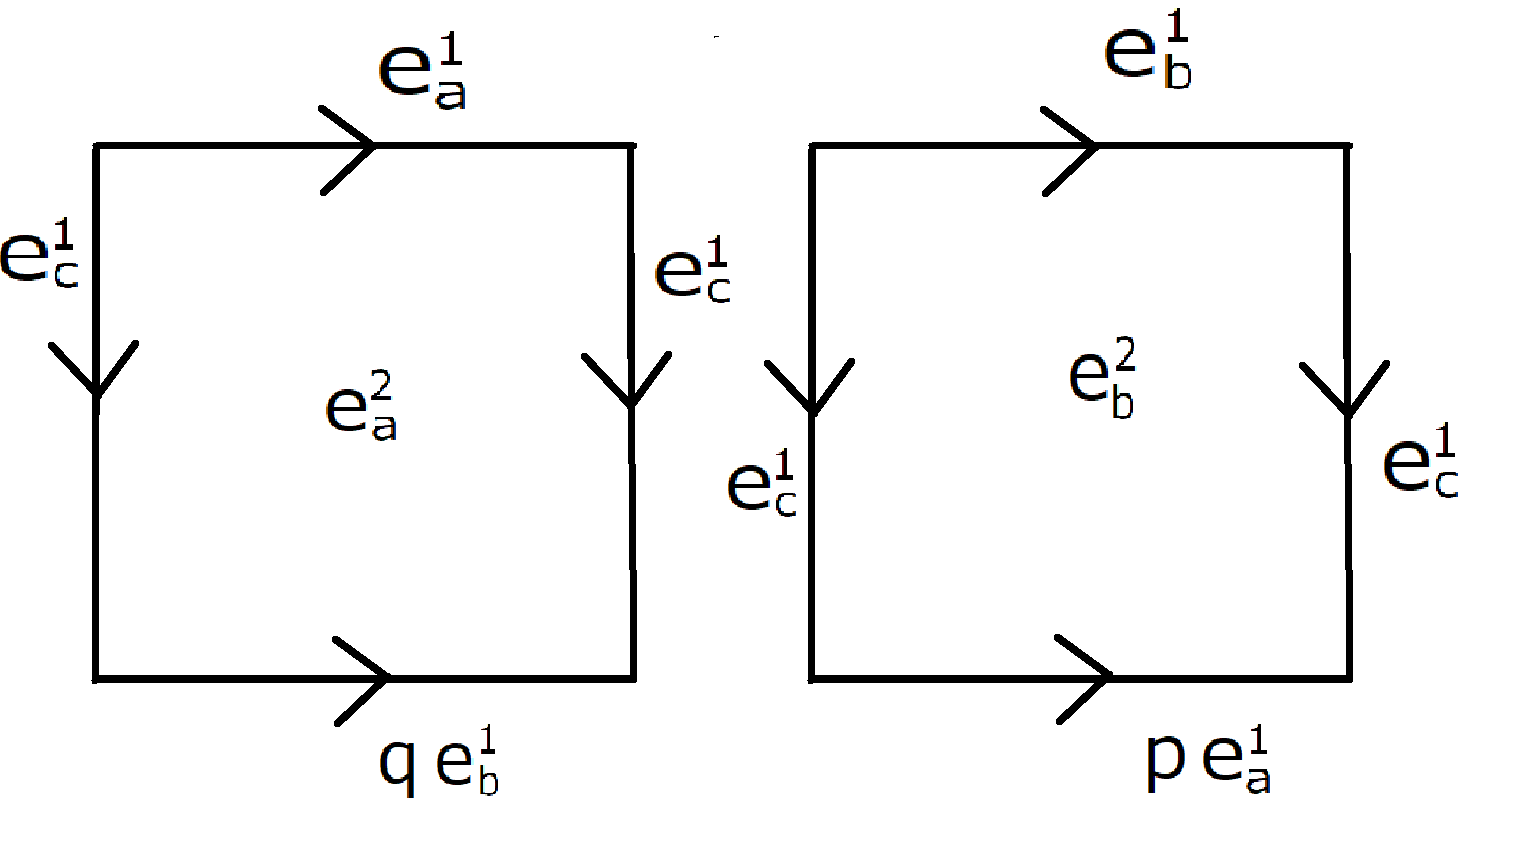
\includegraphics[width=5cm]{H31expert05_02.png}
\end{center}

のような状況になっているので
\[
\del(e_a^2) = e_a^1 - qe_b^1 \quad \del(e_b^2) = e_b^1 - pe_a^1
\]
である。したがって$\del$は次の行列
\[
\del = \pmat{
1 & -p \\
-q & 1 \\
0 & 0
}
\]
で表される写像である。この行列の階数は$pq =1$のとき$1$でそうでないとき$2$である。よって$pq = 1$のとき
\begin{align*}
  H_1(Y) &= \Z^3 / \Im \del \\
  &= \Z^2 \\
  H_2(Y) &= \Ker \del \\
  &= \Z
\end{align*}
である。$pq \neq 1$ならば
\begin{align*}
  H_1(Y) &= \Z^3 / \Im \del \\
  &= (a \Z \oplus  b \Z \oplus c \Z)  / (a - qb, b - pa) \\
  &= (a \Z \oplus  b \Z )  / ( (1-pq)a, b - pa) \oplus c \Z \\
  &= \Z / (1-pq)\Z \oplus \Z \\
  H_2(Y) &= \ker \del \\
  &= 0
\end{align*}
である。以上により求めるホモロジーは、$pq = 1$のとき
\[
H_i(Y) = \begin{cases}
\Z &(i=0,2) \\
\Z^2 &(i=1) \\
0 &(\text{otherwise})
\end{cases}
\]
であり、$pq \neq 1$のとき
\[
H_i(Y) = \begin{cases}
\Z &(i=0) \\
\Z / (pq-1)\Z \oplus \Z &(i=1) \\
0 &(\text{otherwise})
\end{cases}
\]
\end{sol}
